\documentclass[a0paper, portrait]{tikzposter}
\usepackage[utf8]{inputenc}
\usepackage{adjustbox}

%%%%%%%%%%%%%%%%%%%%%%%%
%  table env for tkiz  %
%%%%%%%%%%%%%%%%%%%%%%%%
\newcounter{tablecounter}
\newenvironment{tikztable}[1][]{
  \def \rememberparameter{#1}
  \vspace{10pt}
  \refstepcounter{tablecounter}
  \begin{center}
  }{
    \ifx\rememberparameter\@empty
    \else
    \\[10pt]
    {\small Tab.~\thetablecounter: \rememberparameter}
    \fi
  \end{center}
}
%%%%%%%%%%%%%%%%%%%%%%
 
\title{The Genetic Architecure of Human Aggression}
\author{Robert M. Porsch}
\date{\today}
%\institute{Center of Genomic Science}
%\titlegraphic{\includegraphics{1d.jpg}}
 
\usetheme{Simple}
 
\begin{document}
 
\maketitle


\begin{columns}
  \column{0.5}
  \block{Introduction}{ 
    \begin{itemize}
      \item Aggression has beneficial and harmful consequences 
      \item A heritable trait (50\% to 80\%)
      \item Potential sex differences in the genetic architecture are unclear
      \item Specific genetic loci remain unidentified
      \item Unknown genetic overlap with related phenotypes
    \end{itemize}
  }

  % Aim 
    %\block{Aim}{
    %  \begin{itemize}
    %    \item Identification of \textbf{genetic loci} associated with impulsive Aggression and Risk Taking
    %    \item Investigate the \textbf{genetic overlap} between aggression and related phenotypes
    %    \item Explore \textbf{causal connection} among behavioral phenotypes
    %  \end{itemize}
    %}

    % Methods and Samples
    \block{Description of Samples}{
      \adjustbox{valign=t}{
      \begin{minipage}{0.49\linewidth}
        \textbf{The Netherlands Twin Register (NTR):}\\
        \begin{itemize}
          \item ages 7, 10 and 12
          \item Child Behavior Checklist (CBCL)
          \item 10,765 twin pairs
        \end{itemize}
      \end{minipage}
    }
      \adjustbox{valign=t}{
      \begin{minipage}{0.49\linewidth}
        \textbf{Twin Early Development Study (TEDS):}\\
        \begin{itemize}
          \item ages 7, 9 and 12
          \item Strength and Difficulties Questionnaire (SDQ)
          \item 6,897 twin pairs
        \end{itemize}
      \end{minipage}
    }
      \adjustbox{valign=t}{
      \begin{minipage}{0.29\linewidth}
        \textbf{The UK BioBank}\\
        \begin{itemize}
          \item 40--69 years old
          \item Aggression was measured on a single yes/no item
          \item All subjects were genotyped
        \end{itemize}
      \end{minipage}
    }
      \adjustbox{valign=t}{
      \begin{minipage}{0.79\linewidth}
        \vspace{2cm}
      \begin{tikztable}[Sample Size and Missingness of UK Biobank]
        \input{tables/descriptive_ukb.tex}
      \end{tikztable}
      \end{minipage}
    }
  }

  \block{Twin Modeling}{
    \begin{itemize}
    \item Heritability ranges between 42\% and 78\%
    \item High Stability of Genetic Factors: \\
      Genetic Correlation NTR:\@ $0.76-0.85$ \\
      Genetic Correlation TEDS:\@ $0.64-0.77$ 
    \item Small but significant quantitative sex differences
    \item Genetic factors are the major source of stability
    \item Shared environmental influence are present, especially in boys
    \end{itemize}
  }
    % Association Results
    \block{Phenotypic Effects}{

      \begin{minipage}{0.49\linewidth}
        \begin{tikzfigure}[Phenotypic Correlations]
          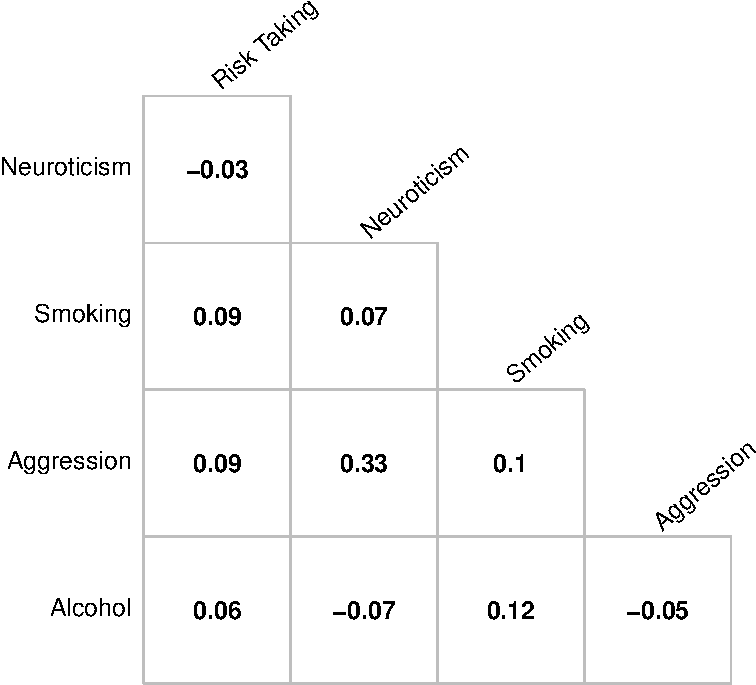
\includegraphics[width=0.99\linewidth]{../ukb_assoc/figure/phenotype/corr_plot_ci.pdf}
        \end{tikzfigure}
      \end{minipage} \hfill
      \begin{minipage}{0.49\linewidth}
        \begin{tikzfigure}[
          Effects of Age (A) and Sex (B) as well as the distrubition of Neuroticisim (C) and drinking behavior (D)
          ]
          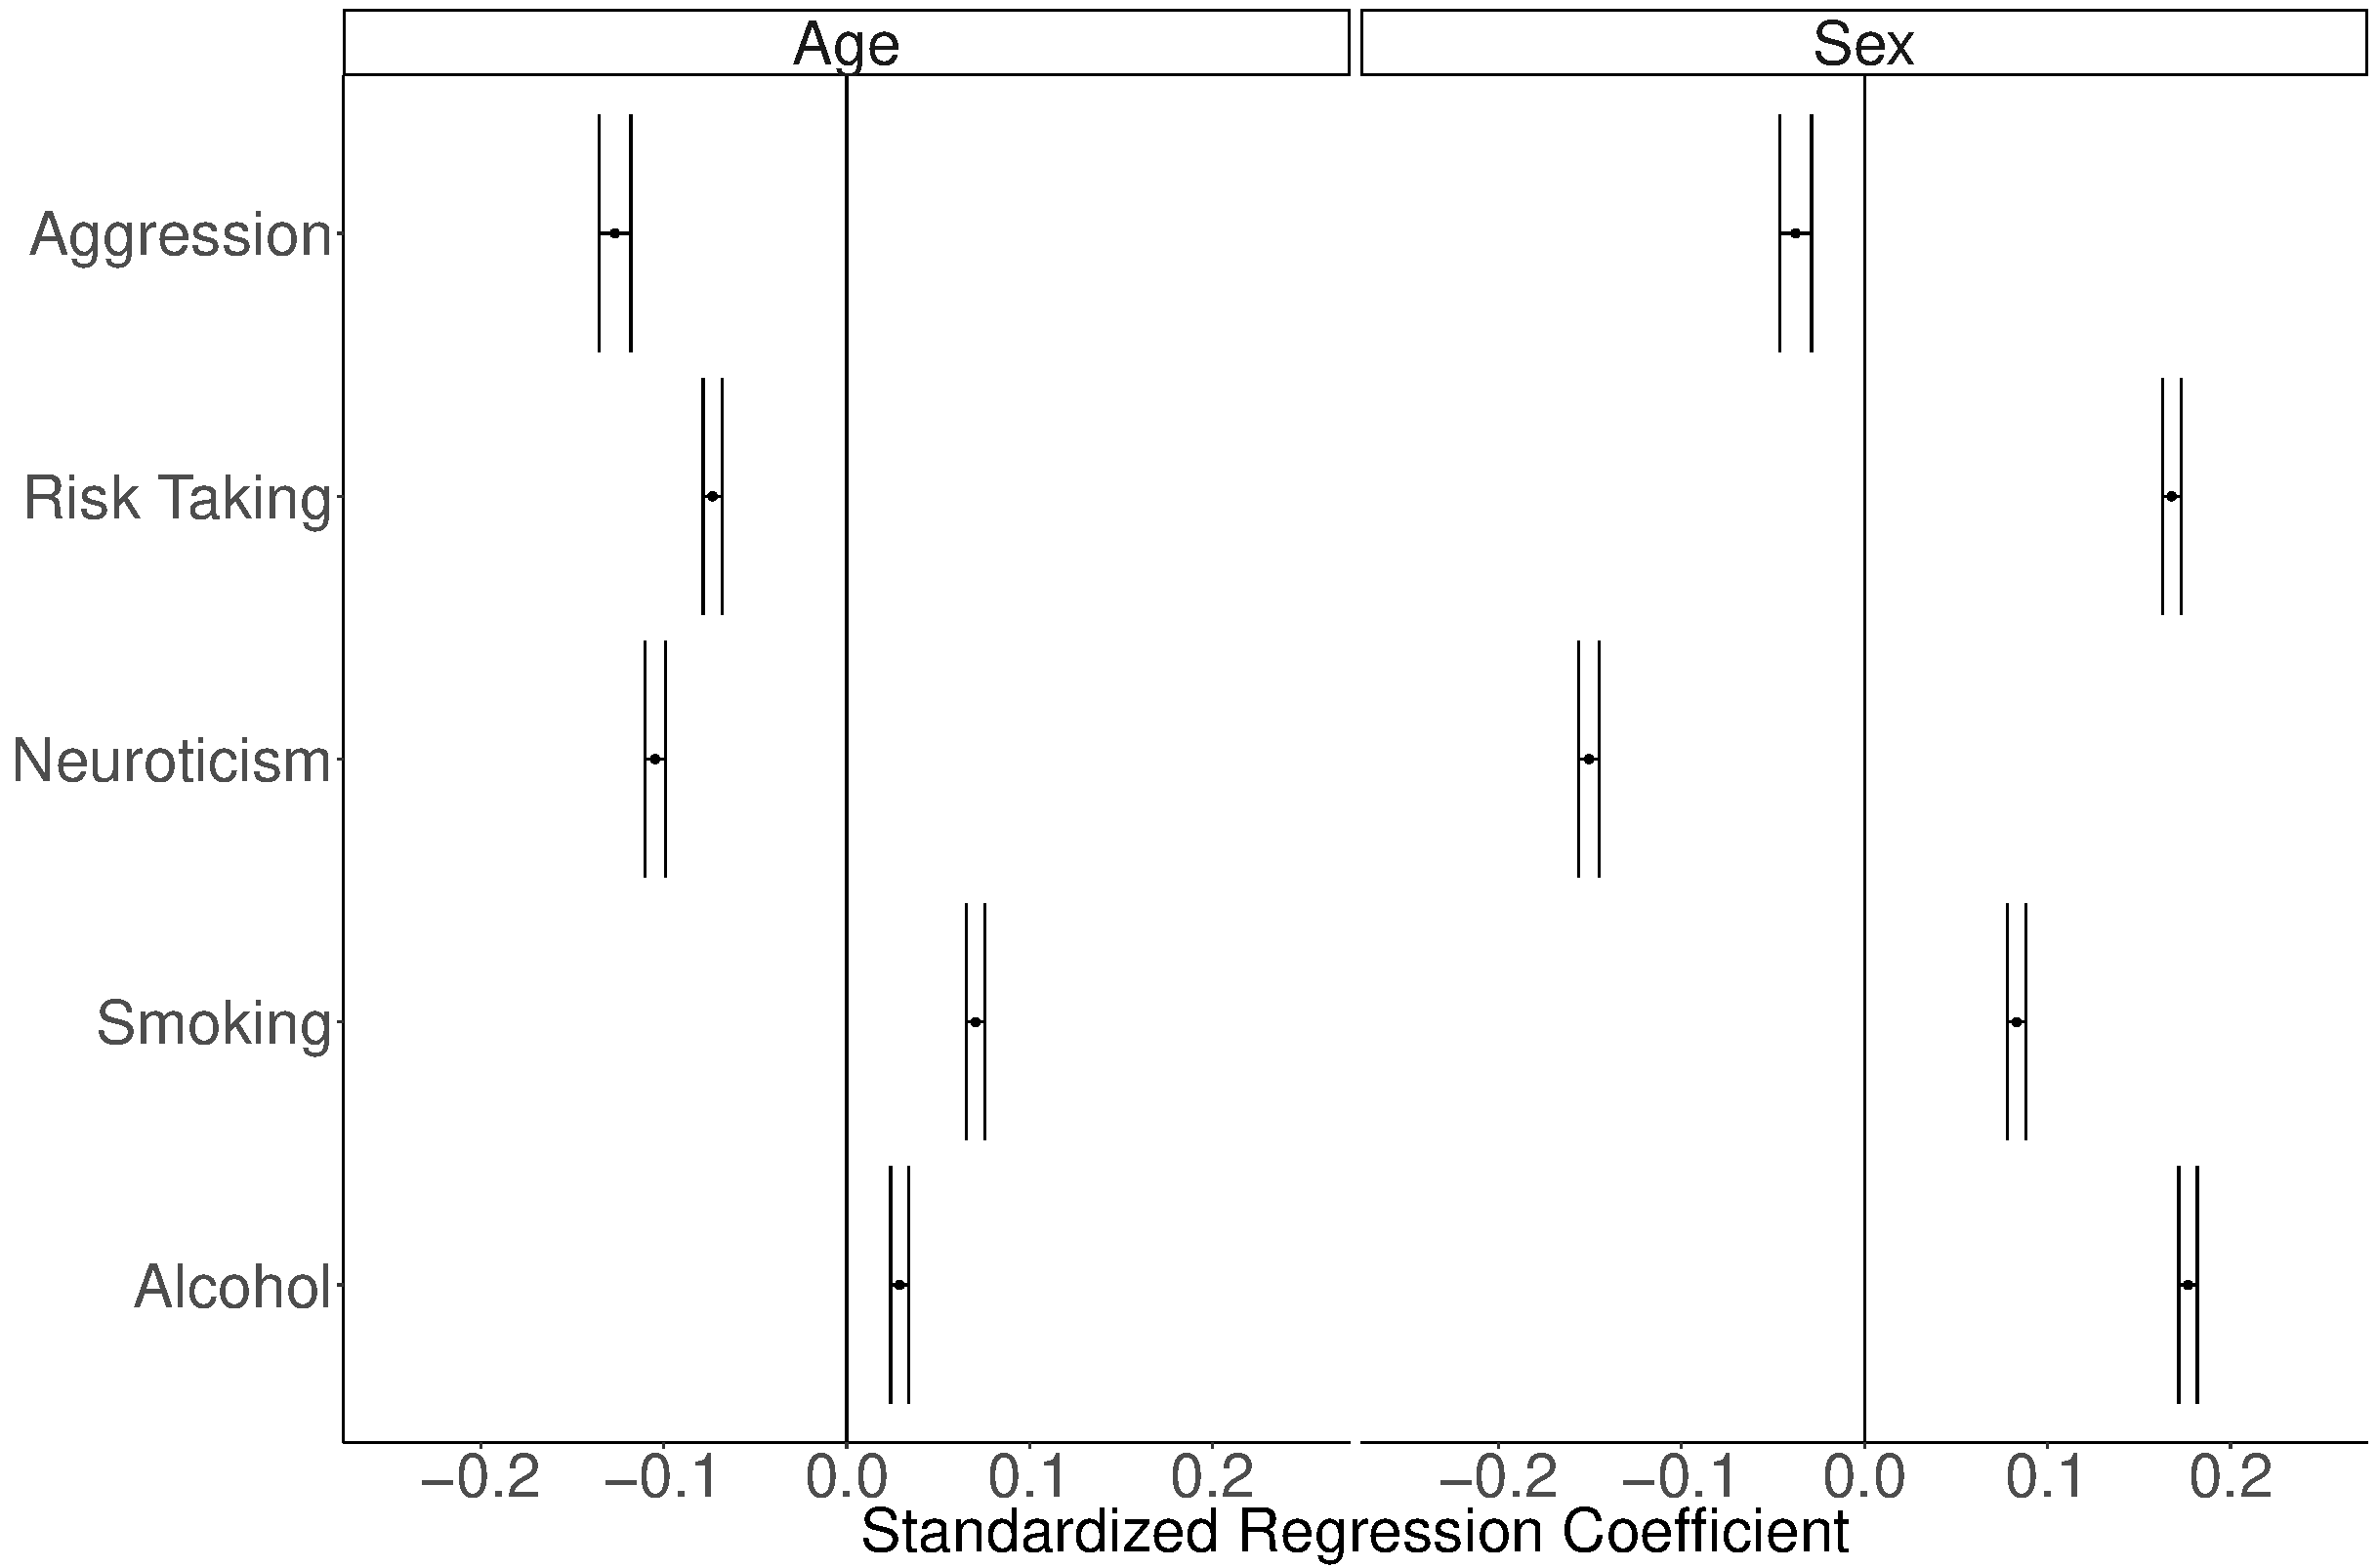
\includegraphics[width=0.99\linewidth]{../ukb_assoc/figure/phenotype/descriptives_plots.pdf}
        \end{tikzfigure}
      \end{minipage}
      \begin{itemize}
        \item Considerable correlation between aggression and neuroticism
        \item Aggression more prominent in male than female
      \end{itemize}
    }
    % Genetic Correlation Matrix

    \block{Conclusion}{
      \begin{itemize}
        \item Heritability: Twin Studies (50\% to 80\%), GWAS (5\%)
        \item limited sample size for aggression
        \item Suggested causal connection between schizophrenia and aggression \& risk taking
        \item independent replication of findings needed
      \end{itemize}
    }

  \column{0.5}

    \block{Genome Wide Association Study}{
      \begin{itemize}
        \item No Genome-wide significant signal was identified
        \item Improved sample size or better phenotyping required
      \end{itemize}
      \begin{minipage}{0.49\linewidth}
        \begin{tikzfigure}
          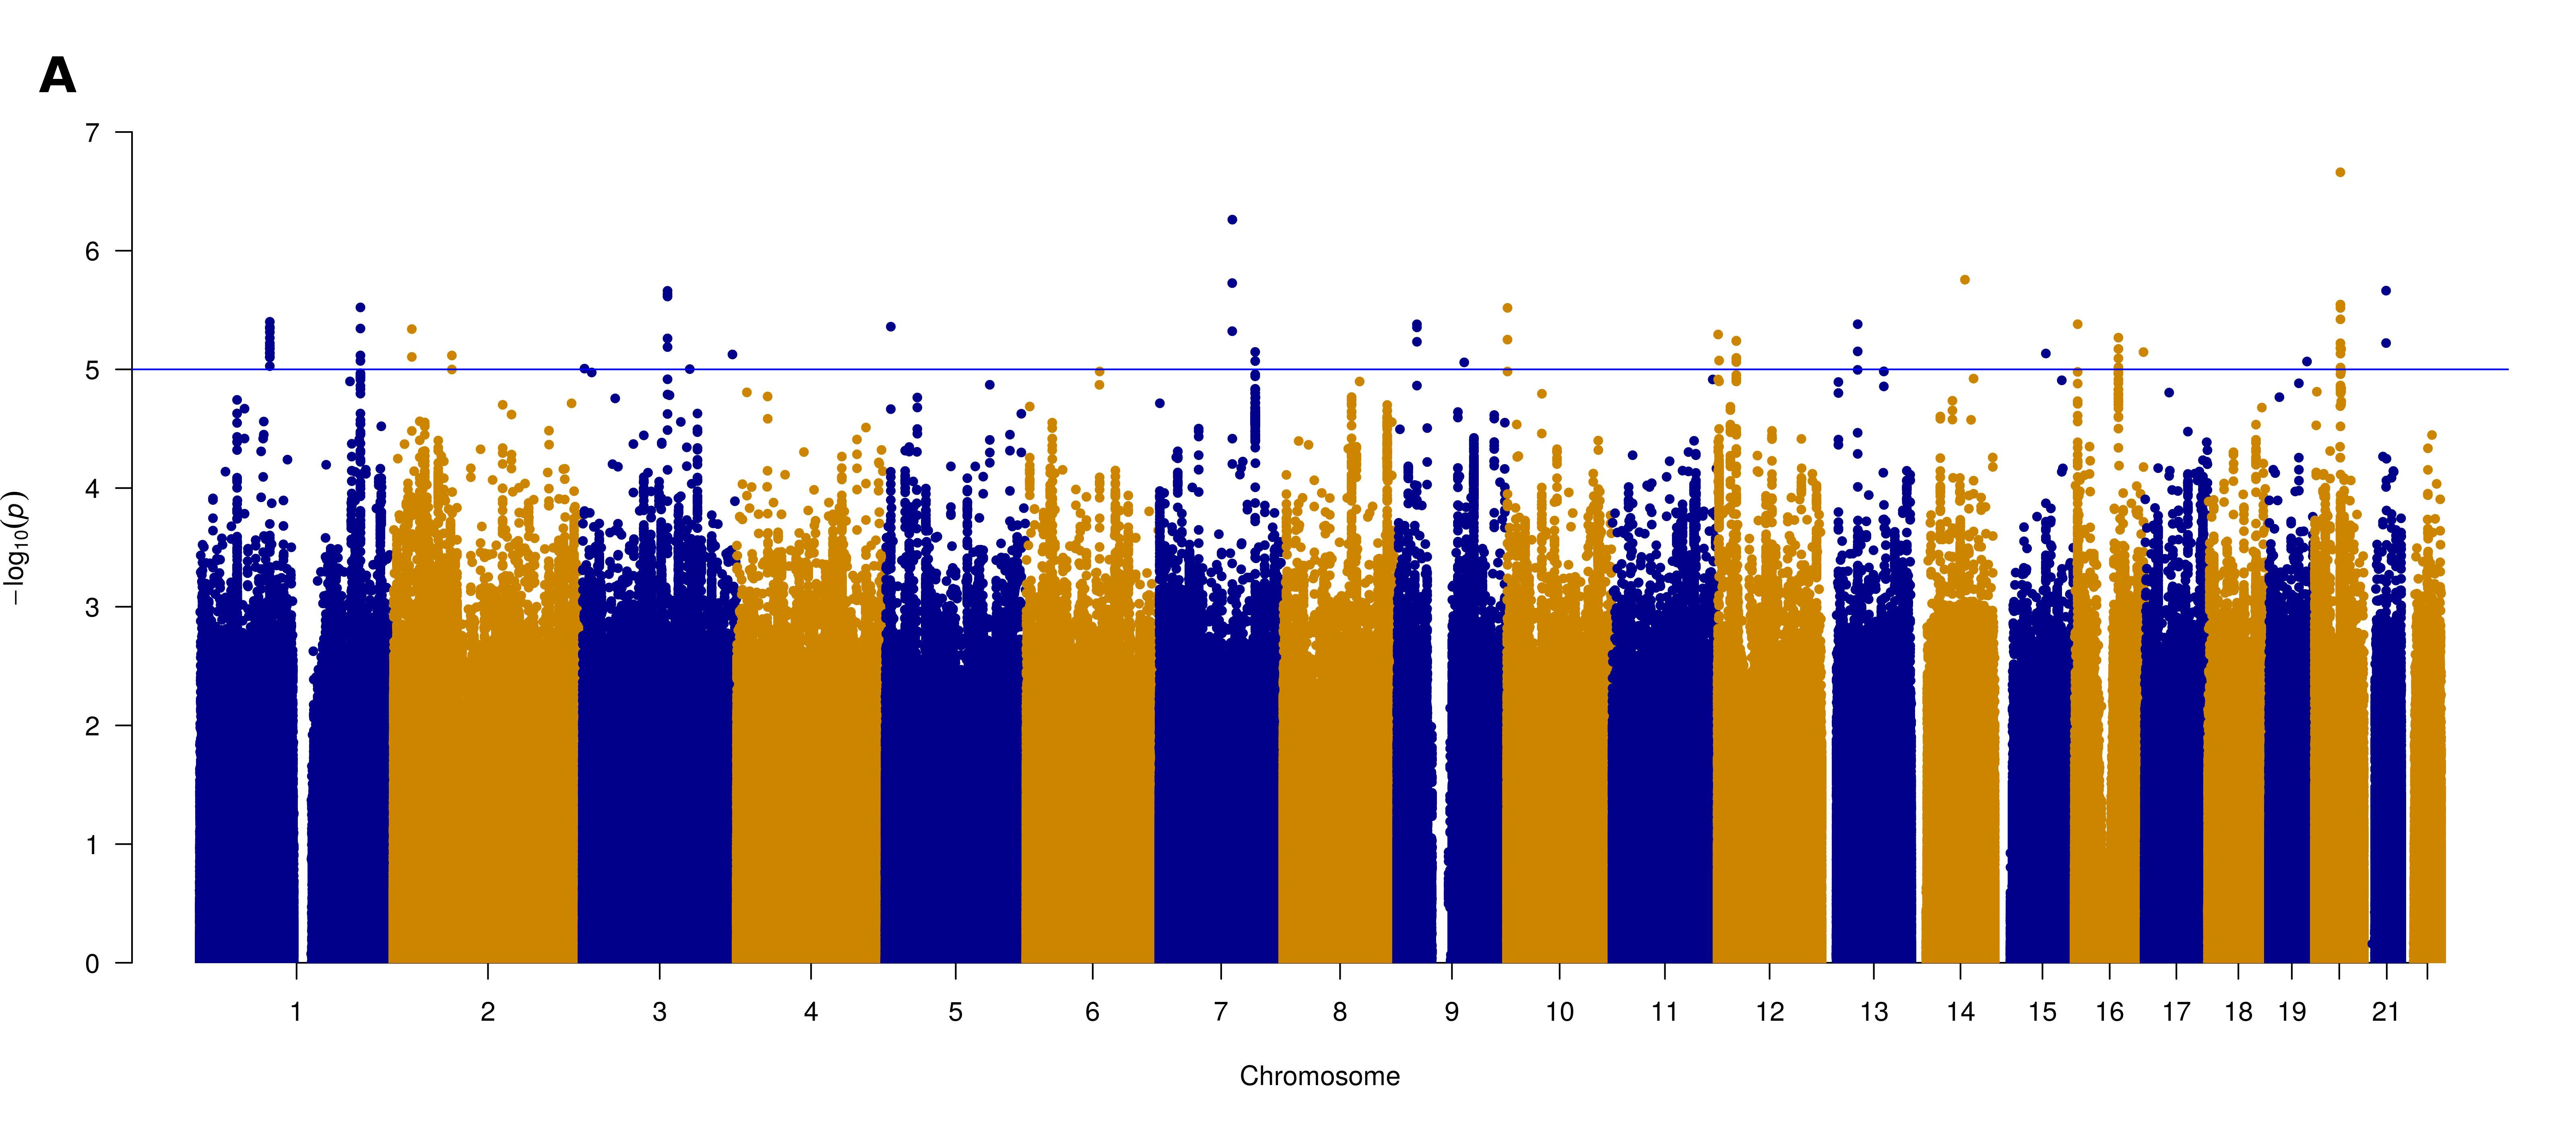
\includegraphics[width=0.8\linewidth]{../ukb_assoc/figure/manhatten_plots/agg_manhatten_color_2_A.jpeg}
        \end{tikzfigure}
      \end{minipage}
      \begin{minipage}{0.49\linewidth}
        \begin{tikzfigure}
          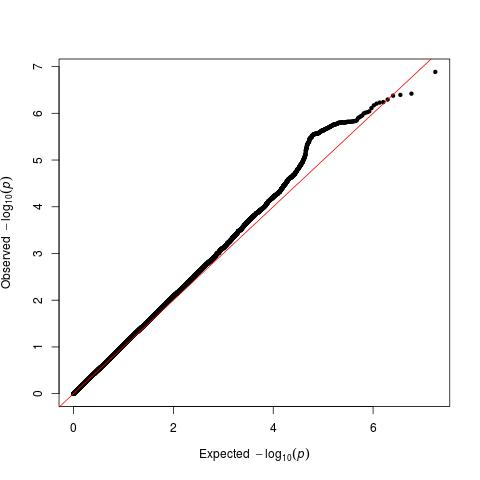
\includegraphics[width=0.7\linewidth]{{../ukb_assoc/figure/qq_plots/qq_plot_4526}.jpeg}
        \end{tikzfigure}
      \end{minipage}
    }

    \block{Genetic Correlations}{
      \begin{tikzfigure}[Genetic Correlations within the UKB]
        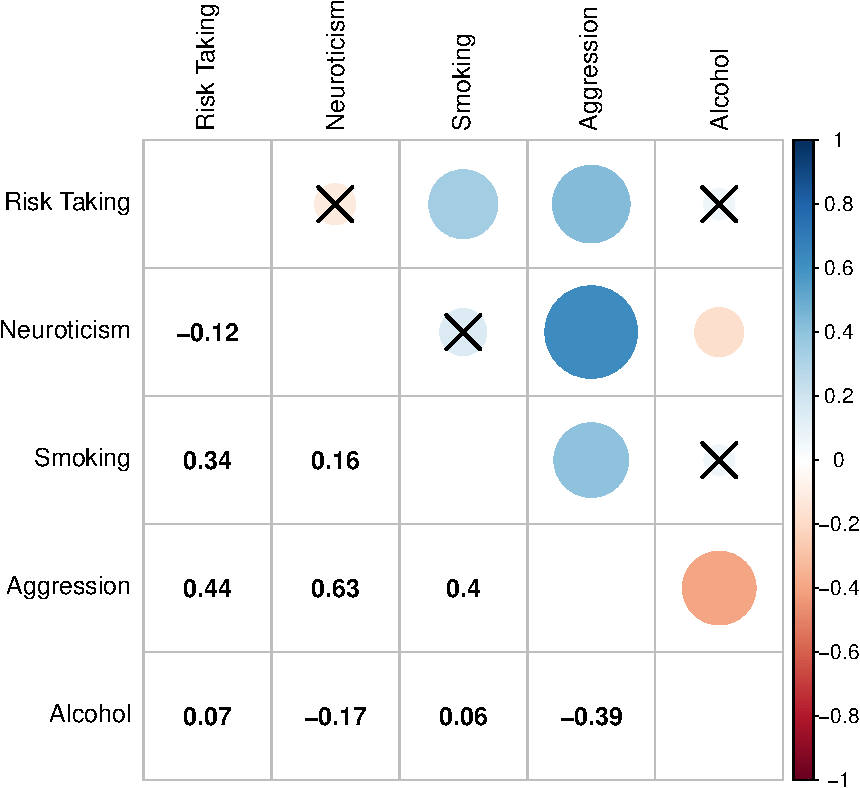
\includegraphics[width=0.65\linewidth]{../ukb_assoc/figure/genetic_corr/gcorr_plot_circle_full_se.pdf}
      \end{tikzfigure}
      \begin{itemize}
        \item Large genetic correlations between aggression and neuroticism
        \item Considerable negative genetic correlations between aggression and alcohol consumption
      \end{itemize}
    }

    % Phenotypic Effects

    % MR
    \block{Estimating Causality: Mendelian Randomization}{
      \textbf{What is Mendelian Randomization?}
        \begin{itemize}
          \item Infers potential causal effects from observational data 
          \item Natural randomized control trial
          \item Testing for a causal connection between psychiatric disorders and aggression as well as risk taking
        \end{itemize}
      \begin{tikzfigure}[
        Estimated causal effect of psychiatric disorders on impulsive aggression and risk taking.
        The effect size of the causal effect $\beta$ is displayed on the y-axis, while used Mendelian randomization methods are on the x-axis.
        SZ, Schizophrenia; MDD, Major Depressive Disorder; DS, Depressive Symptom's; BP, Bipolar Disorder.
        (A) Effect of psychiatric disorders on impulsive aggression.
        (A) Effect of psychiatric disorders on risk taking.
        ]\label{fig:overall_mr_effect}
        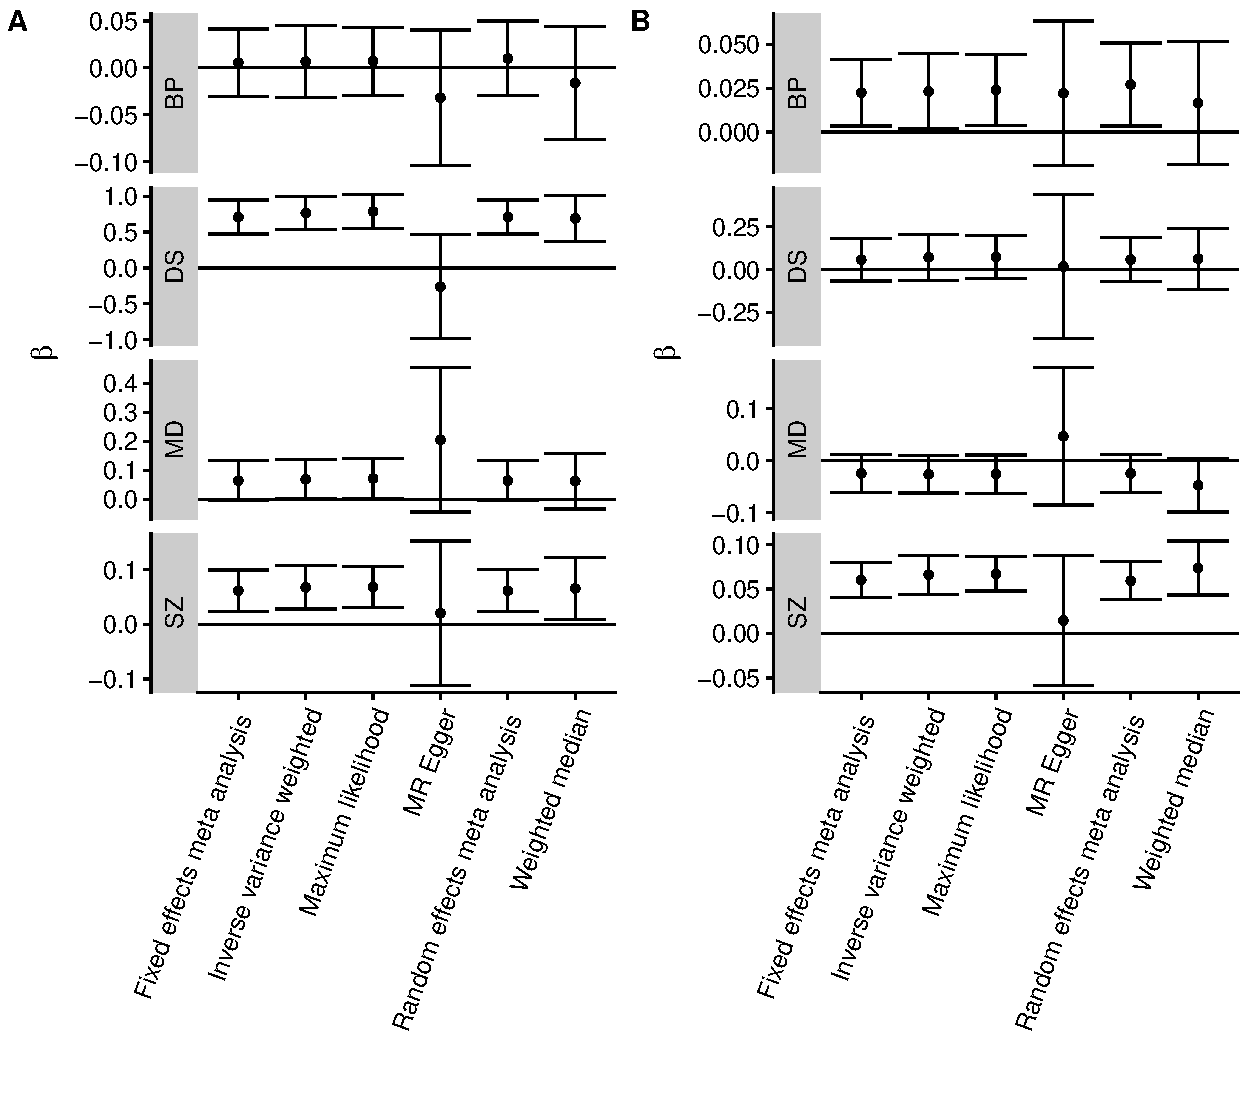
\includegraphics[width=0.6\linewidth]{../ukb_psychiatric/figures/overall_mr_effect.pdf}
      \end{tikzfigure}
      \textbf{Results:}
      \begin{itemize}
        \item Estimated causal effects are small
        \item Some indication for a causal connection betwee SZ and aggression/risk taking
      \end{itemize}
    }

\end{columns}

\end{document}
